\documentclass[10pt]{article}
\usepackage[margin=2.4cm]{geometry}
\usepackage{graphicx,booktabs,xcolor,hyperref,enumitem}
\hypersetup{colorlinks=true,linkcolor=blue!60!black,urlcolor=blue!60!black}
\setlist{nosep,leftmargin=1.4em}
\newcommand{\code}[1]{\texttt{\small #1}}
\title{\vspace{-1.2em}P8B Profiling: Qwen3-8B-Base on ASearcher (32-turn, top-5, 16k)\\
\large vanilla vs.\ synchronous partial rollout, GRPO vs.\ turnPPO\vspace{-0.6em}}
\author{Agentic-RL-CA rung-3 --- branch \code{sync-partial-rollout-poc}}
\date{2026-07-29/30 \; (SF time)}
\begin{document}
\maketitle
\vspace{-1.6em}

\section*{TL;DR}
All four configs run end-to-end on one 8$\times$H100 worker. The partial-rollout PoC is
\textbf{functionally correct} (T1/T3-lite resume identity byte-exact; group-atomic release
invariants hold in every cycle; zero stale drops) and gives \textbf{1.5--1.6$\times$}
overall throughput (2.2--2.5$\times$ on generation). However, \textbf{no configuration meets
the $\sim$3-day/arm gate at the full protocol budget}: projected 150-step wall-clock is
13.3\,d (GRPO vanilla) / 8.9\,d (GRPO partial) / 20.3\,d (turnPPO vanilla, pre-fix estimate)
/ 12.8\,d (turnPPO partial). Decision options in \S5; \textbf{no arm was auto-launched}.

\section{Setup}
Qwen3-8B-Base, RL-from-base, ASearcher Base-35k \emph{unfiltered}, wiki-18/e5 top-5,
one 5k-char \code{<information>} block per turn (never discarded), full
\code{<think>}+\code{<search>} responses retained in history, 32-turn nominal horizon,
16k prompt with \emph{clean context-overflow termination}, 1024-token responses,
256$\times$5 = 1280 trajectories/step, \code{MICRO\_BSZ}=1. Partial rollout:
\code{cycle\_turns}=8, \code{max\_age}=4, uid-group-atomic release, no off-policy
correction (per-row \code{policy\_version} recorded). Profiling: 2 steps/config vanilla,
4 cycles/config partial (turnPPO-partial cycle 4 cut by the 6\,h per-config timeout;
3 clean cycles suffice). Runs: \code{p8bprof\_*} in wandb project
\href{https://wandb.ai/rainyfields/ca-rung3-8b-asearcher}{\code{ca-rung3-8b-asearcher}}.

\section{Correctness of the partial-rollout PoC}
\begin{itemize}
\item \textbf{T1 resume identity} (scripted actions, live retriever): prompts restored from
snapshots byte-identical to the uninterrupted reference, before \emph{and} after a
post-restore step (done-flags included). \textbf{T3-lite}: \code{reset\_partial([])}
$\equiv$ vanilla reset. Log: \code{t1\_resume\_identity.log}.
\item \textbf{Conservation invariants} hold exactly in all 7 partial cycles observed:
carried + fresh = released + pending + held; released always divisible by group size 5.
\item \textbf{Staleness}: mean open-group age 0.35--0.45 cycles; \code{dropped\_stale\_groups}=0
throughout ($\le$1 policy-version lag for most resumed segments).
\end{itemize}

\section{Throughput and memory}
\begin{center}
\begin{tabular}{lrrrr}
\toprule
 & GRPO vanilla & GRPO partial & turnPPO vanilla$^\dagger$ & turnPPO partial\\
\midrule
step/cycle wall-clock (mean, s) & 7652 & 3728 & 11681 & 4041\\
generation share (s) & 3961 & 1591 & 5740 & 1585\\
update share (s) & 2086 & 1262 & 4850 & 2009\\
step-seconds / completed traj & 5.98 & \textbf{4.00} & 9.13 & \textbf{5.76}\\
projected 150-step arm (days) & 13.3 & 8.9 & 20.3 & 12.8\\
peak mem alloc (GB) & 85.2 & 70--85 & OOM@KV0.6$^\dagger$ & fits @KV0.5+offload\\
\bottomrule
\end{tabular}
\end{center}
\noindent$^\dagger$turnPPO vanilla crashed at cycle 2's vLLM \code{wake\_up(kv\_cache)} under
KV fraction 0.6 with the colocated 8B critic; its numbers above are from its single
completed step. A retry under the fixed posture (KV 0.5 + critic CPU offload, matching
turnPPO partial) is in flight; expect update share to grow somewhat from offload.

\begin{center}
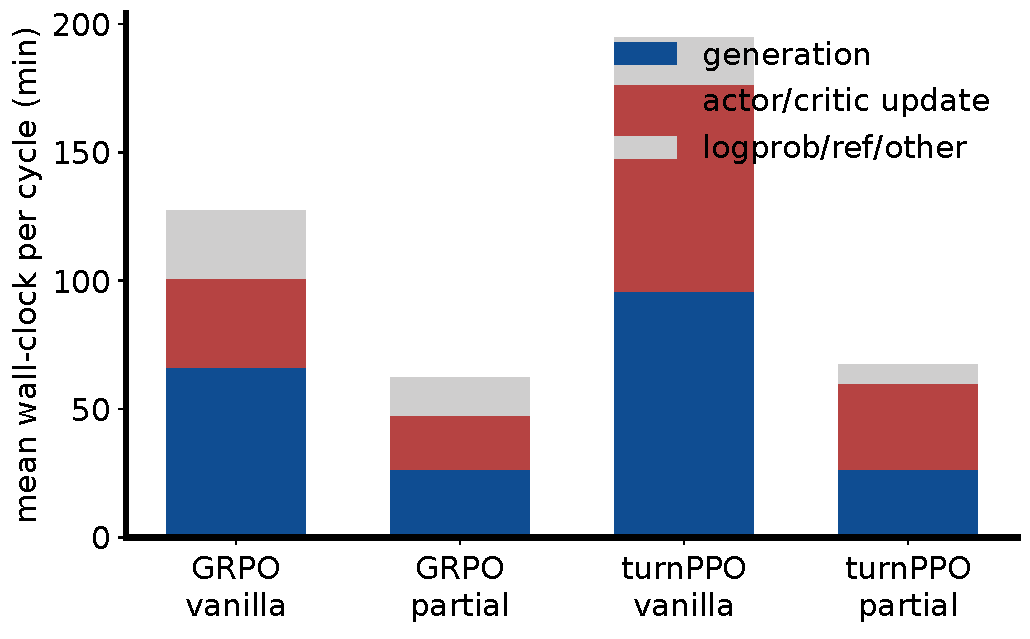
\includegraphics[width=0.48\linewidth]{assets/fig_step_breakdown}\hfill
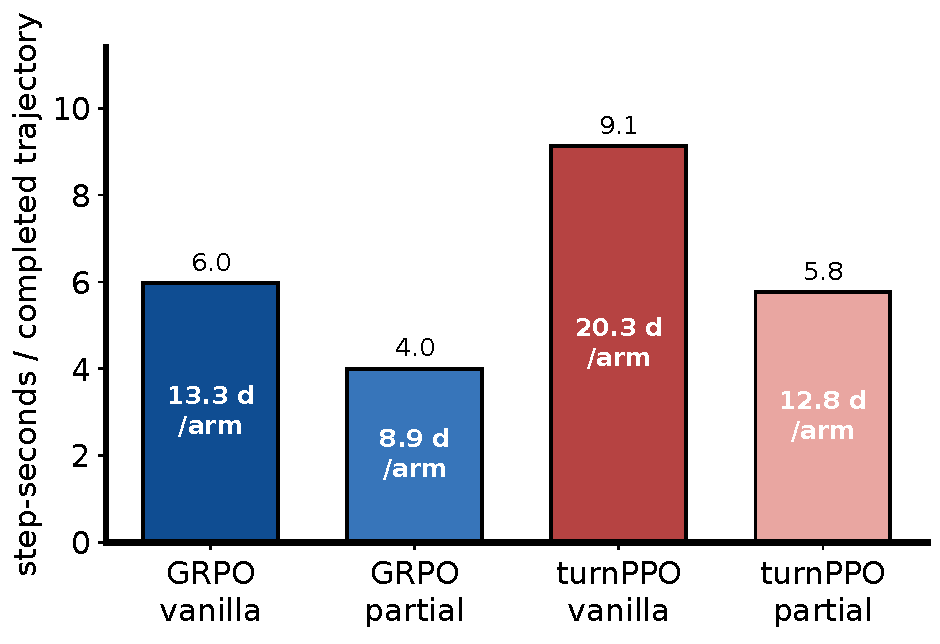
\includegraphics[width=0.48\linewidth]{assets/fig_throughput}\\[0.4em]
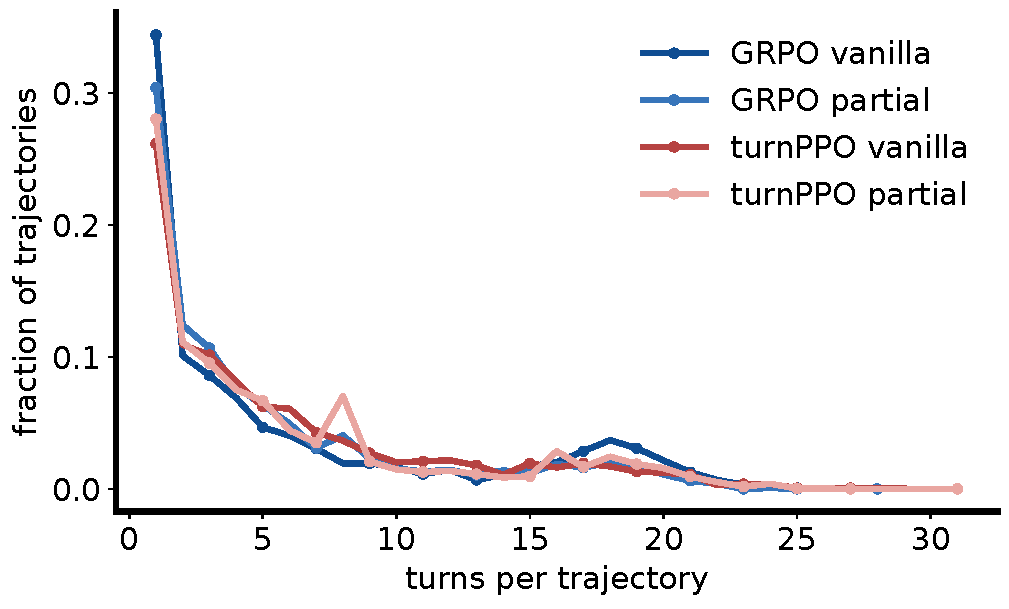
\includegraphics[width=0.48\linewidth]{assets/fig_turns_hist}\hfill
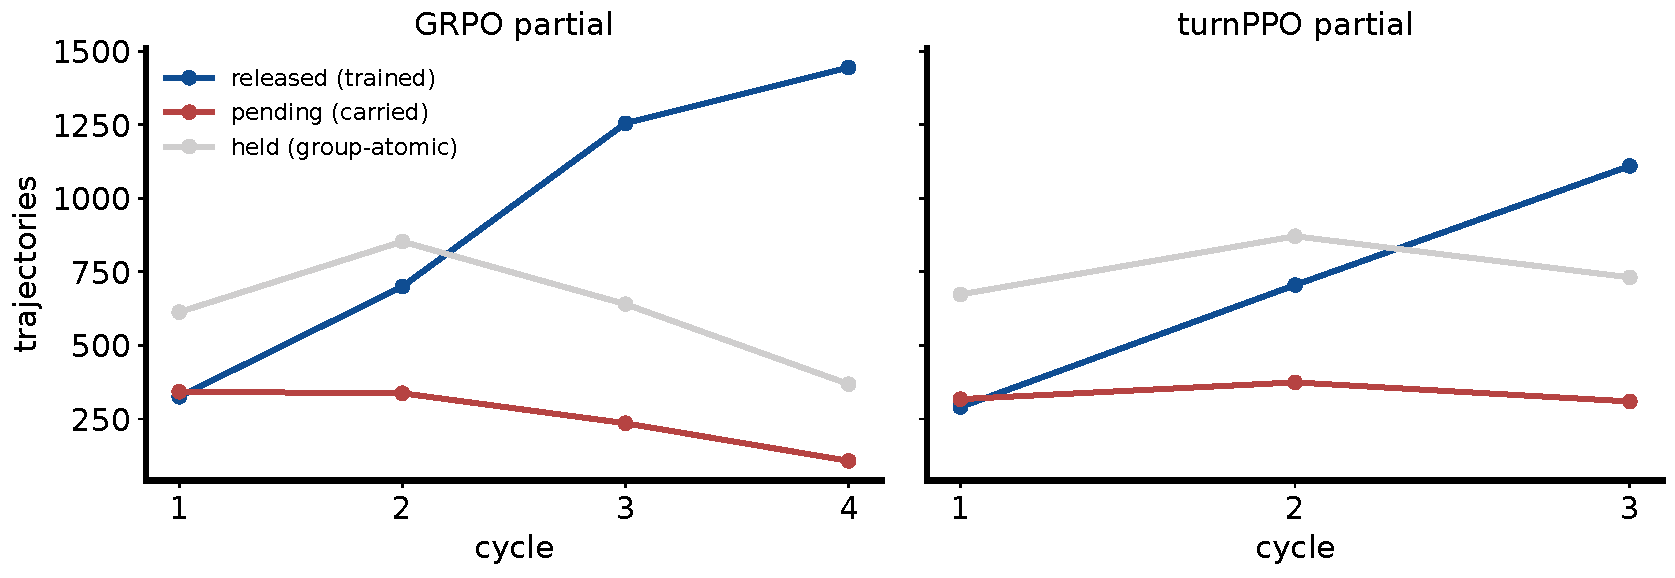
\includegraphics[width=0.48\linewidth]{assets/fig_partial_dynamics}
\end{center}

Generation is the straggler-bound share and is where partial rollout pays: 2.2--2.5$\times$.
Updates scale with trained tokens (identical either way), diluting overall gain to
1.5--1.6$\times$. Buffer dynamics (bottom-right) show steady state after cycle 2:
$\sim$1250--1450 released/cycle at 1280-slot pool, pending 100--370.

\section{Trajectory behaviour (RL-from-base sanity)}
\begin{itemize}
\item \textbf{Grammar compliance out of the box}: step-0 greedy val em \textbf{0.199}
(512 unfiltered questions), avg 8.2 turns, 7.6 searches/traj, 0\% unterminated ---
the base 8B uses the tool grammar zero-shot (the 4B-Instruct greedy baseline was 0.010).
Training valid-action ratio 0.315 at step 1 (temp 1.0), entropy 2.57$\to$1.97 by step 2.
\item \textbf{Length wall}: mean 5.3--6.1 turns, max 26 ($<$32): the 16k prompt binds first,
as designed. Ctx-terminate produced clean endings; residual prompt-clip 0.5\% (char
prefilter tail --- tighten threshold before headline runs).
\item \textbf{Caps}: 5k info-block cap hits 3--8\% of retrievals; 1024-token response cap
hits 24--37\% of turns (long base-model thinks).
\item \textbf{Train success} 0.16--0.20 at temp 1.0 (unfiltered data; parametric shortcut
present by design --- cf.\ the filtered-4B step-0 of 0.008).
\end{itemize}

\section{Decision needed (no auto-launch)}
The grilled go-criterion ``$<\sim$3 days/arm'' fails for every config, so the two 150-step
arms were \textbf{not} launched. Options, combinable:
\begin{enumerate}
\item \textbf{Partial rollout for both arms} (8.9\,d GRPO / 12.8\,d turnPPO): systems-faithful
to ASearcher, but couples the algorithm comparison to the PoC's uncorrected staleness (R2).
\item \textbf{Cut steps to 75} ($\approx$4.5\,d / 6.4\,d with partial): halves optimization
budget; 4B curves suggest most movement happens by step 75.
\item \textbf{Shrink batch or group} (e.g.\ 128$\times$5): halves step cost, halves
trajectories/update; breaks strict budget-matching with the 4B arms.
\item \textbf{Accept the wall-clock} for vanilla arms (13--20\,d each) --- cleanest science,
slowest calendar, occupies 2 of $\sim$6 quota slots throughout.
\end{enumerate}

\section*{Reproduce}
\code{scripts/asearcher/p8b\_profile\_worker.sh} (worker; \code{ONLY\_CFG} to subset),
\code{analyze\_profiling.py} + \code{make\_figures.py} (this folder). Raw per-turn dumps:
HDFS \code{logs/p8b\_profile/rollout\_*.jsonl.zst}. Design doc:
\code{docs/design/2026-07-29\_sync\_partial\_rollout.md}.
\end{document}
